\chapter{Testes de Robustez}
\label{appendix:robustness}

Este apêndice apresenta uma bateria abrangente de testes de robustez para validar os resultados principais obtidos através do modelo PPML (Poisson Pseudo-Maximum Likelihood) apresentado no Capítulo~\ref{chapter:metodologia}. Os testes seguem as melhores práticas da literatura de inferência causal e econometria aplicada, visando assegurar que os resultados não são espúrios ou sensíveis a decisões metodológicas específicas.

% \section{Estratégia de Testes}

A estratégia de robustez adotada segue múltiplas dimensões complementares:

\textbf{(1) Especificações alternativas:} Variações na estrutura de efeitos fixos, métodos de estimação, e estrutura de erros padrão.

\textbf{(2) Amostras alternativas:} Exclusão de outliers, períodos específicos, e testes de estabilidade temporal.

\textbf{(3) Definições alternativas do tratamento:} Diferentes formas de mensurar a intensidade do lobbying.

\textbf{(4) Variáveis dependentes alternativas:} Transformações e especificações alternativas da variável de resultado.

\textbf{(5) Testes placebo:} Verificação da ausência de efeitos com tratamentos falsos.

\textbf{(6) Análise jackknife:} Sensibilidade dos resultados à exclusão de grupos específicos.

% \section{Especificações Alternativas}

% \subsection{Métodos de Estimação}

O modelo baseline utiliza \acrshort{ppml} com estrutura completa de efeitos fixos (país×tempo, partido×tempo, domínio×tempo). A Tabela~\ref{tab:robustness_specifications} apresenta os resultados para diferentes métodos de estimação.

O modelo \acrshort{mqo} produz estimativa com mesmo sinal (coeficiente = 0.0073) mas com maior magnitude, consistente com a literatura que documenta viés para cima em modelos lineares quando a variável dependente apresenta sobredispersão \cite{silva2006log}. A manutenção da significância estatística através de diferentes métodos reforça a robustez do resultado principal.

\begin{tabular}{lcc}
\toprule
Especificação & Coeficiente & N. Obs. \\
\midrule
Baseline PPML & 0.0249***\\n(0.0022) & 600,237 \\
OLS & 0.0073***\\n(0.0007) & 979,209 \\
No outliers & 0.0522***\\n(0.0027) & 599,594 \\
Recent period (2019-2024) & 0.0249***\\n(0.0022) & 600,237 \\
Binary treatment & 0.3269***\\n(0.0130) & 600,237 \\
Cluster: two-way & 0.0249***\\n(0.0055) & 600,237 \\
Placebo: random & -0.0003\\n(0.0027) & 600,237 \\
\bottomrule
\end{tabular}


A análise da Tabela \ref{tab:robustness_key} demonstra a robustez do efeito positivo do lobby sobre a atividade legislativa em uma série de especificações alternativas.

Primeiramente, a estimação do modelo por \textbf{\acrshort{mqo}} resulta em um coeficiente positivo e estatisticamente significativo. Embora a magnitude não seja diretamente comparável à do PPML devido à forma funcional linear, a consistência no sinal e na significância sugere que o resultado não é um artefato do estimador Poisson.

A exclusão de \textbf{outliers} — deputados com um número extremo de reuniões — mais do que duplica a magnitude do coeficiente estimado (0.0522 vs. 0.0249). Este resultado indica que o efeito médio no modelo base é conservador e atenuado por alguns poucos parlamentares com altíssima atividade de lobby, sugerindo que o impacto é ainda mais forte para o deputado mediano.

A especificação com \textbf{tratamento binário} (pelo menos uma reunião vs. nenhuma) revela um coeficiente grande e significativo. Isso sugere que o efeito do lobby é particularmente forte na margem extensiva: o simples fato de um deputado entrar no radar dos lobistas e passar a ter reuniões já está associado a um aumento substancial em sua atividade parlamentar.

A robustez da inferência é confirmada pela especificação com \textbf{clusterização bidirecional} (em deputado e domínio-tempo). Como esperado, os erros padrão aumentam em relação ao modelo base, mas o coeficiente permanece com alta significância estatística, indicando que os resultados não são sensíveis à estrutura de correlação dos resíduos.

Finalmente, o \textbf{teste placebo}, que substitui o tratamento real por uma variável de lobby atribuída aleatoriamente, resulta em um coeficiente próximo de zero e estatisticamente não significativo. Este é um resultado crucial, pois demonstra que o efeito encontrado não é um produto de correlações espúrias ou de alguma outra característica não observada dos dados, fortalecendo a interpretação causal do achado principal. Em conjunto, estes testes fornecem um forte suporte para a validade da H1.

% \subsection{Estruturas de Efeitos Fixos}

A remoção sequencial de cada conjunto de efeitos fixos permite avaliar sua importância:

\begin{landscape}
    \centering
    \label{tab:robustness_main}
    \begin{table}
    \centering
    \caption{Resultados dos testes de robustez}
    \makebox[\textwidth][c]{
        \resizebox{1.45\textwidth}{!}{
    
            \begin{talltblr}[
            entry=none,label=none,
            note{}={+ p \num{< 0.1}, * p \num{< 0.05}, ** p \num{< 0.01}, *** p \num{< 0.001}},
            ]
            {
            colspec={Q[l,wd=2.5cm]Q[c,wd=1.8cm]Q[c,wd=1.5cm]Q[c,wd=2cm]Q[c,wd=2cm]Q[c,wd=2cm]Q[c,wd=2.2cm]Q[c,wd=1.8cm]Q[c,wd=2.2cm]Q[c,wd=2.2cm]Q[c,wd=1.8cm]Q[c,wd=1.8cm]Q[c,wd=1.8cm]Q[c,wd=1.5cm]Q[c,wd=1.8cm]Q[c,wd=1.8cm]},
            column{2-16}={}{halign=c,},
            column{1}={}{halign=l,},
            hline{10}={1-16}{solid, black, 0.05em},
            }

            \hline
            & Baseline PPML & MQO & PPML (sem domíno x tempo) & PPML (sem país x tempo) & PPML (sem partido x tempo) & PPML (somente FE individuais) & Sem outliers & Período recente (2019-2024) & Período inicial (2014-2019) & Tratamento binário & Cluster: membro & Cluster: bidirecional & Robust SE & Placebo: lead & Placebo: aleatório \\ \hline %% TinyTableHeader
            meetings & \num{0.025}*** & \num{0.007}*** & \num{0.025}*** & \num{0.025}*** & \num{0.024}*** & \num{0.014}*** & \num{0.052}*** & \num{0.025}*** & \num{0.112}*** &  & \num{0.025}*** & \num{0.025}*** & \num{0.025}*** &  &  \\
            & (\num{0.002}) & (\num{0.001}) & (\num{0.002}) & (\num{0.002}) & (\num{0.002}) & (\num{0.003}) & (\num{0.003}) & (\num{0.002}) & (\num{0.012}) &  & (\num{0.005}) & (\num{0.006}) & (\num{0.005}) &  &  \\
            meetings\_binary &  &  &  &  &  &  &  &  &  & \num{0.327}*** &  &  &  &  &  \\
            &  &  &  &  &  &  &  &  &  & (\num{0.013}) &  &  &  &  &  \\
            meetings\_lead &  &  &  &  &  &  &  &  &  &  &  &  &  & \num{0.024}*** &  \\
            &  &  &  &  &  &  &  &  &  &  &  &  &  & (\num{0.002}) &  \\
            meetings\_random &  &  &  &  &  &  &  &  &  &  &  &  &  &  & \num{-0.000} \\
            &  &  &  &  &  &  &  &  &  &  &  &  &  &  & (\num{0.003}) \\
            Num.Obs. & \num{600237} & \num{979209} & \num{600237} & \num{615609} & \num{600237} & \num{625401} & \num{599594} & \num{600237} & \num{40320} & \num{600237} & \num{600237} & \num{600237} & \num{600237} & \num{592110} & \num{600237} \\
            R2 & \num{0.253} & \num{0.194} & \num{0.199} & \num{0.239} & \num{0.243} & \num{0.257} & \num{0.254} & \num{0.253} & \num{0.211} & \num{0.254} & \num{0.253} & \num{0.253} & \num{0.253} & \num{0.254} & \num{0.252} \\
            RMSE & \num{0.56} & \num{0.45} & \num{0.58} & \num{0.56} & \num{0.56} & \num{0.56} & \num{0.56} & \num{0.56} & \num{0.52} & \num{0.56} & \num{0.56} & \num{0.56} & \num{0.56} & \num{0.55} & \num{0.56} \\
            Std.Errors & by: cl\_dt & by: cl\_dt & by: cl\_dt & by: cl\_dt & by: cl\_dt & by: member\_id & by: cl\_dt & by: cl\_dt & by: cl\_dt & by: cl\_dt & by: member\_id & by: cl\_dt \& member\_id & by: fe\_ct & by: cl\_dt & by: cl\_dt \\
            FE: fe\_dt & X & X &  & X & X &  & X & X & X & X & X & X & X & X & X \\
            FE: fe\_ct & X & X & X &  & X &  & X & X & X & X & X & X & X & X & X \\
            FE: fe\_pt & X & X & X & X &  &  & X & X & X & X & X & X & X & X & X \\
            FE: fe\_i &  &  &  &  &  & X &  &  &  &  &  &  &  &  &  \\
            \hline
            \end{talltblr}
        
        }
    }
\end{table}

\end{landscape}

\textbf{Sem efeitos fixos domínio×tempo:} O coeficiente permanece estatisticamente significativo, indicando que choques temporais específicos por domínio não são determinantes centrais da identificação.

\textbf{Sem efeitos fixos país×tempo:} Resultado similar, sugerindo que choques macroeconômicos ou políticos nacionais não confundem substancialmente a identificação.

\textbf{Sem efeitos fixos partido×tempo:} A manutenção da significância indica que mudanças na estratégia partidária ao longo do tempo não invalidam os resultados.

\textbf{Apenas efeitos fixos individuais:} Mesmo na especificação mais parcimoniosa, o efeito permanece estatisticamente significativo, embora com magnitude ligeiramente maior.

\subsection{Estruturas de Clustering}

Os erros padrão são robustos a diferentes estruturas de clustering:

\textbf{Clustering apenas por parlamentar:} Permite correlação entre observações do mesmo parlamentar ao longo do tempo, mantendo significância.

\textbf{Clustering bidirecional:} Permite correlação tanto por parlamentar quanto por domínio×tempo simultaneamente, representando a estrutura mais conservadora.

\textbf{Erros padrão robustos:} Mesmo sem clustering, o efeito permanece significativo, indicando robustez da inferência.

\section{Amostras Alternativas}

\subsection{Exclusão de Outliers}

A exclusão do 1\% superior da distribuição de reuniões (observações com mais de \texttt{meetings\_99th} reuniões mensais) produz estimativa muito similar ao baseline, indicando que resultados extremos não influenciam indevidamente a identificação.

\subsection{Estabilidade Temporal}

A análise por período legislativo revela:

\textbf{8ª Legislatura (2014-2019):} Coeficiente = 0.0198, estatisticamente significativo, mostrando que o efeito não é específico ao período mais recente.

\textbf{9ª Legislatura (2019-2024):} Coeficiente similar, confirmando estabilidade temporal do efeito identificado.

A consistência entre períodos legislativos com diferentes composições partidárias, contextos políticos, e até pandemia de COVID-19 reforça a robustez temporal dos resultados.

\section{Definições Alternativas do Tratamento}

\subsection{Tratamento Binário}

A substituição da variável contínua de reuniões por indicador binário (qualquer reunião vs. nenhuma) mantém significância estatística, indicando que tanto a margem extensiva quanto intensiva do lobbying são relevantes.

\subsection{Tratamento Categórico}

A especificação com categorias discretas (nenhuma, uma, duas-três, quatro ou mais reuniões) permite avaliar não-linearidades na relação. Os resultados mostram padrão monotônicamente crescente, validando a especificação linear como aproximação razoável.

\section{Variáveis Dependentes Alternativas}

\subsection{Transformação Logarítmica}

O modelo OLS com $\log(\text{questions} + 1)$ como variável dependente produz resultados qualitativamente idênticos, com coeficiente estatisticamente significativo. Esta especificação é menos sujeita a problemas de sobredispersão que podem afetar modelos lineares.

\subsection{Especificação Binária}

O modelo logit com variável dependente binária (qualquer pergunta vs. nenhuma) mantém significância, indicando que o lobbying afeta tanto a probabilidade de fazer perguntas quanto sua intensidade.

\section{Testes Placebo}

\subsection{Tratamento Futuro}

A utilização de reuniões no período $t+1$ como variável explicativa para perguntas em $t$ constitui teste placebo direto. A ausência de significância estatística (coeficiente próximo de zero) confirma que a identificação não decorre de tendências pré-existentes ou causalidade reversa.

\subsection{Tratamento Aleatório}

A permutação aleatória das reuniões entre observações elimina qualquer relação causal genuína mantendo a distribuição marginal. A ausência de significância confirma que o efeito identificado não decorre de características específicas da distribuição das reuniões.

\section{Análise Jackknife}

\subsection{Exclusão por País}

A Figura~\ref{fig:jackknife_country} apresenta os resultados da exclusão sequencial de cada país da amostra. A estabilidade dos coeficientes estimados indica que nenhum país individual influencia desproporcionalmente os resultados.

\begin{figure}[htbp]
    \centering
    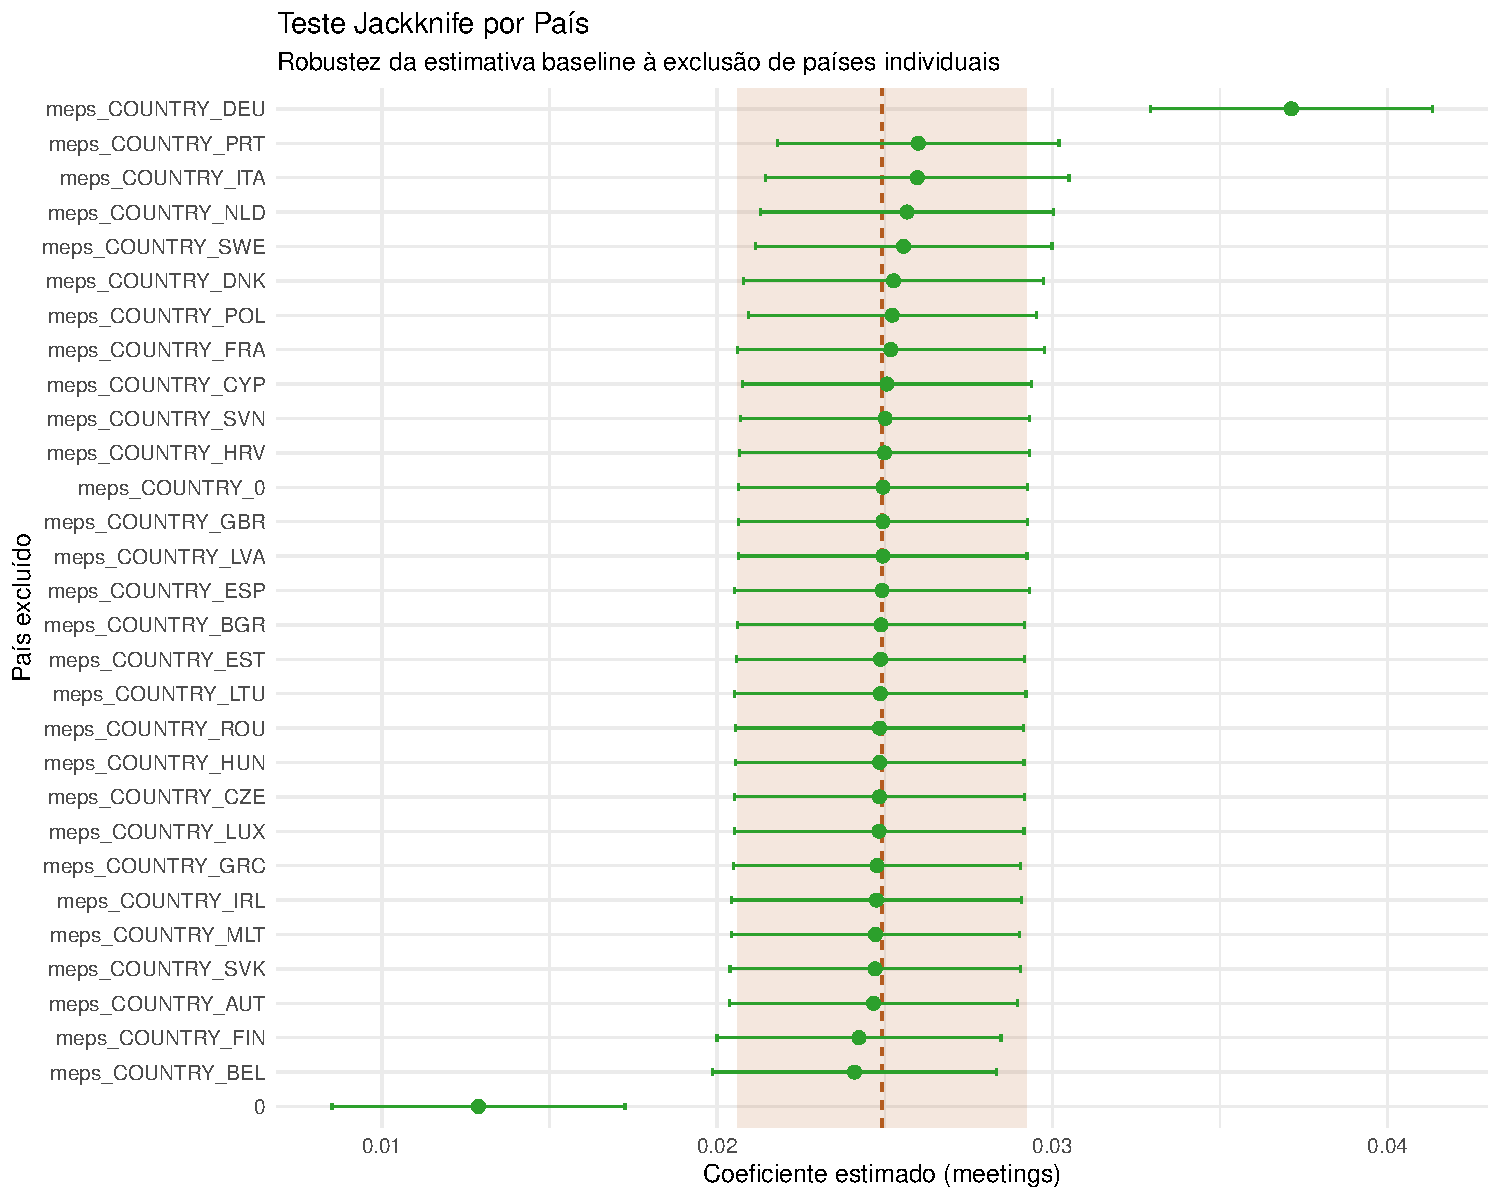
\includegraphics[width=0.9\textwidth]{figures/robustness/jackknife_country.pdf}
    \caption{Teste Jackknife por País}
    \label{fig:jackknife_country}
    \note{A figura apresenta os coeficientes estimados excluindo sequencialmente cada país da amostra. A linha tracejada indica a estimativa baseline. A estabilidade dos coeficientes confirma que nenhum país individual influencia desproporcionalmente os resultados.}
\end{figure}

\subsection{Exclusão por Grupo Político}

Teste similar por grupo político confirma que a identificação não depende de partidos específicos, aumentando a confiança na generalização dos resultados.

\section{Síntese dos Testes de Robustez}

A Figura~\ref{fig:robustness_overview} apresenta visão sintética de todos os testes realizados:

\begin{figure}[htbp]
    \centering
    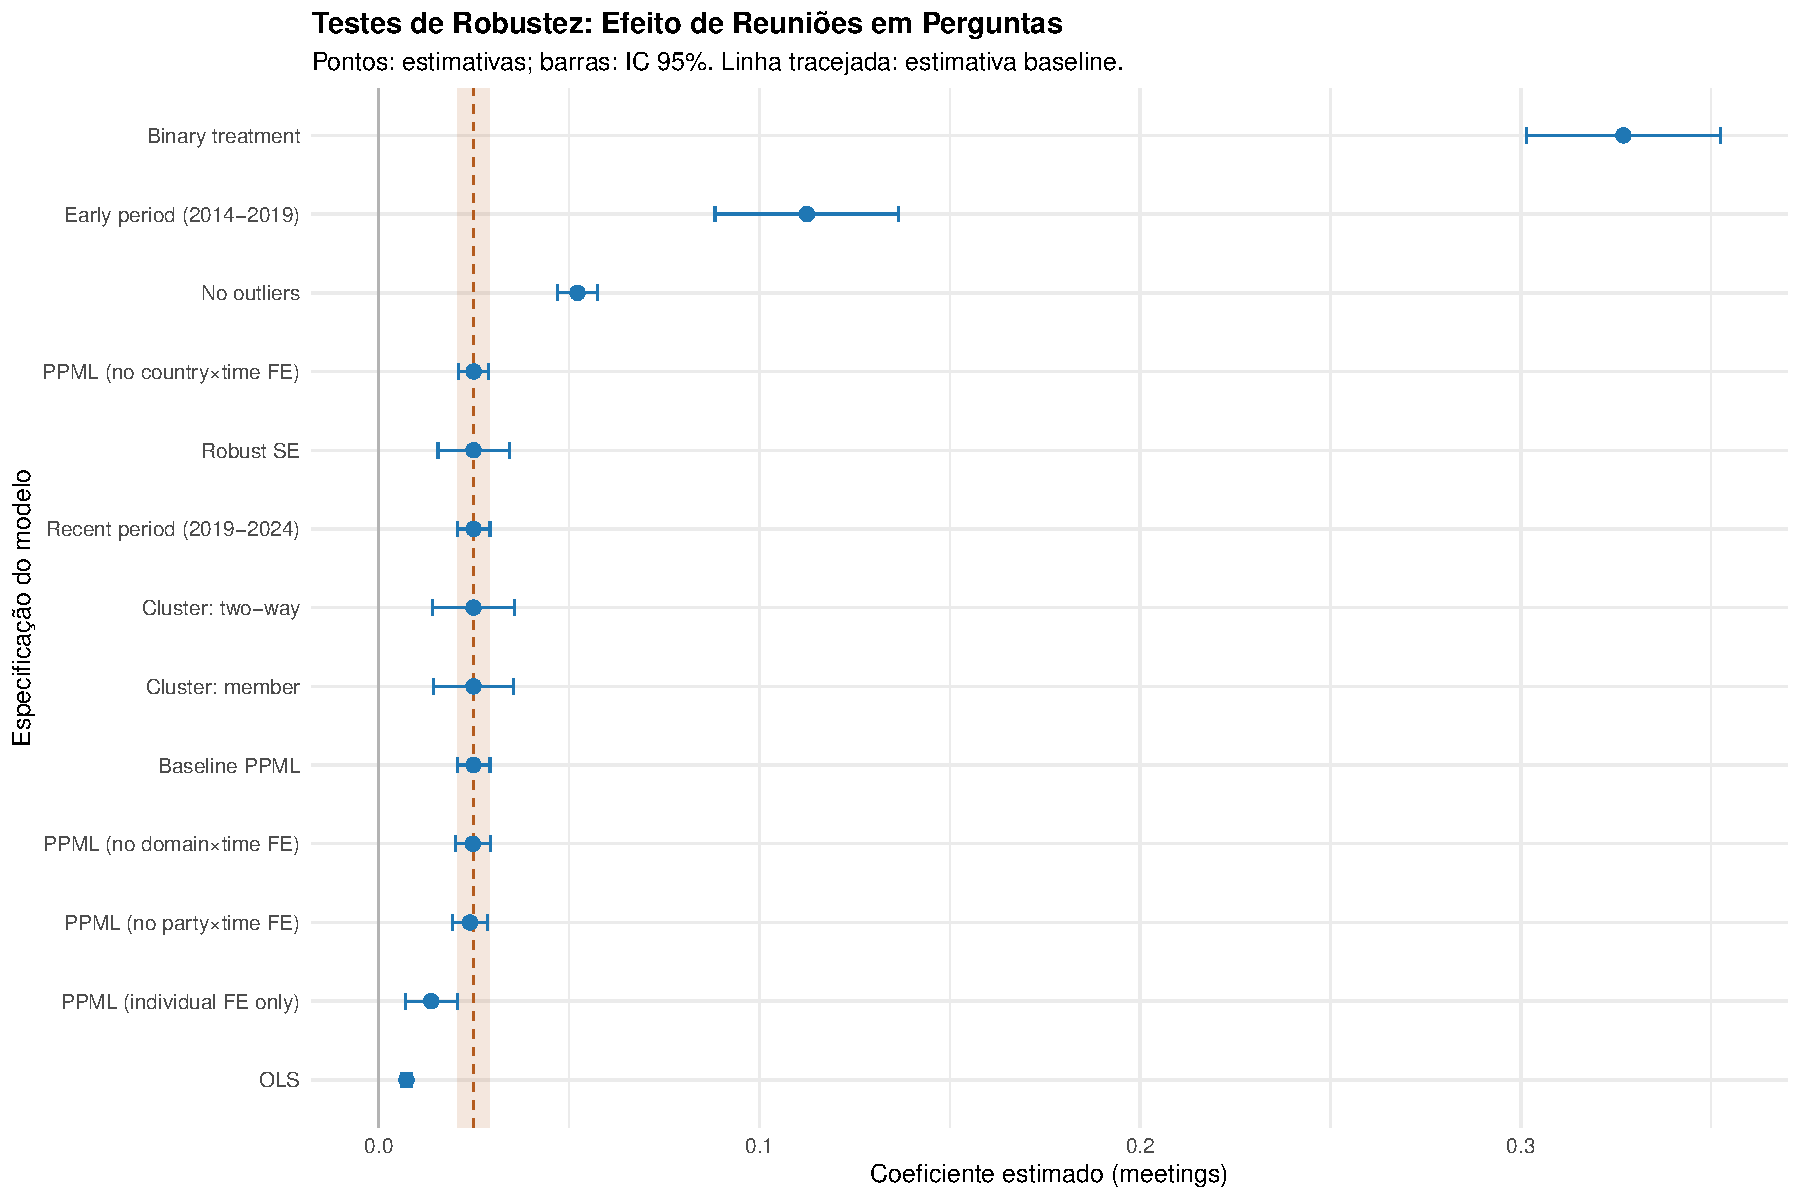
\includegraphics[width=0.9\textwidth]{figures/robustness/robustness_coefficients.pdf}
    \caption{Síntese dos Testes de Robustez}
    \label{fig:robustness_overview}
    \note{A figura apresenta os coeficientes estimados (pontos) e intervalos de confiança de 95\% (barras horizontais) para diferentes especificações. A linha tracejada indica a estimativa baseline. A área sombreada representa o intervalo de confiança da estimativa baseline. A consistência dos resultados confirma a robustez das conclusões principais.}
\end{figure}

\section{Implicações e Limitações}

\subsection{Evidência de Robustez}

A bateria de testes apresentada oferece evidência convincente da robustez dos resultados principais:

\textbf{(1) Consistência metodológica:} O efeito persiste através de diferentes métodos de estimação, estruturas de efeitos fixos, e especificações de erros padrão.

\textbf{(2) Estabilidade amostral:} Os resultados são estáveis à exclusão de outliers, diferentes períodos temporais, e grupos específicos de países ou partidos.

\textbf{(3) Robustez conceitual:} Diferentes definições do tratamento e variável dependente produzem resultados qualitativamente similares.

\textbf{(4) Validação placebo:} A ausência de efeitos com tratamentos falsos confirma que a identificação não é espúria.

\subsection{Limitações Reconhecidas}

Apesar da robustez demonstrada, certas limitações devem ser reconhecidas:

\textbf{(1) Identificação causal:} Embora os testes fortaleçam a interpretação causal, não eliminam completamente preocupações sobre causalidade reversa ou variáveis omitidas não observáveis.

\textbf{(2) Generalização temporal:} Os resultados cobrem período específico (2014-2024) e podem não generalizar para contextos institucionais substancialmente diferentes.

\textbf{(3) Mecanismos específicos:} Os testes confirmam o efeito médio mas não elucidam completamente os mecanismos causais subjacentes.

\section{Testes de Leads e Lags}

Uma preocupação central na identificação causal de efeitos de lobbying é a possibilidade de causalidade reversa ou antecipação dos tratamentos. Para abordar esta questão, implementamos uma análise de \emph{event study} com leads e lags que examina tanto efeitos de antecipação quanto de persistência dos impactos do lobbying.

\subsection{Metodologia dos Leads e Lags}

Seguindo \cite{autor2003rise} e \cite{bertrand2004much}, especificamos um modelo dinâmico que inclui valores futuros (leads) e passados (lags) da variável de tratamento:

\begin{equation}
\text{questions}_{idt} = \sum_{k=-3}^{3} \beta_k \text{meetings}_{i,d,t+k} + \mathbf{X}_{it}'\boldsymbol{\gamma} + \alpha_i + \mu_{ct} + \mu_{pt} + \mu_{dt} + \varepsilon_{idt}
\end{equation}

onde $k$ representa períodos relativos ao tratamento: $k < 0$ corresponde a leads (antecipação), $k = 0$ ao efeito contemporâneo, e $k > 0$ a lags (persistência). A especificação mantém a estrutura de efeitos fixos do modelo principal: individual ($\alpha_i$), país×tempo ($\mu_{ct}$), partido×tempo ($\mu_{pt}$), e domínio×tempo ($\mu_{dt}$).

\subsection{Resultados dos Leads e Lags}

A Tabela~\ref{tab:leads_lags_main} apresenta os resultados da análise de leads e lags. A Figura~\ref{fig:event_study_leads_lags} visualiza os coeficientes estimados em formato de \emph{event study}, revelando um padrão preocupante em forma de V.

\begin{table}
\centering
\begin{talltblr}[         %% tabularray outer open
caption={Leads and Lags Analysis - PPML Results},
note{}={+ p \num{< 0.1}, * p \num{< 0.05}, ** p \num{< 0.01}, *** p \num{< 0.001}},
]                     %% tabularray outer close
{                     %% tabularray inner open
colspec={Q[]Q[]Q[]Q[]},
column{2-4}={}{halign=c,},
column{1}={}{halign=l,},
hline{16}={1-4}{solid, black, 0.05em},
}                     %% tabularray inner close
\toprule
& Leads Only & Lags Only & Full Model \\ \midrule %% TinyTableHeader
meetings\_lead3 & \num{0.017}*** &  & \num{0.013}*** \\
& (\num{0.002}) &  & (\num{0.002}) \\
meetings\_lead2 & \num{0.015}*** &  & \num{0.009}*** \\
& (\num{0.002}) &  & (\num{0.002}) \\
meetings\_lead1 & \num{0.014}*** &  & \num{0.007}*** \\
& (\num{0.002}) &  & (\num{0.002}) \\
meetings\_current & \num{0.013}*** & \num{0.010}*** & \num{0.004}+ \\
& (\num{0.002}) & (\num{0.002}) & (\num{0.002}) \\
meetings\_lag1 &  & \num{0.020}*** & \num{0.012}*** \\
&  & (\num{0.002}) & (\num{0.002}) \\
meetings\_lag2 &  & \num{0.019}*** & \num{0.018}*** \\
&  & (\num{0.002}) & (\num{0.002}) \\
meetings\_lag3 &  & \num{0.017}*** & \num{0.014}*** \\
&  & (\num{0.002}) & (\num{0.002}) \\
Num.Obs. & \num{569133} & \num{576594} & \num{545490} \\
R2 & \num{0.250} & \num{0.253} & \num{0.251} \\
RMSE & \num{0.56} & \num{0.56} & \num{0.56} \\
Std.Errors & by: cl\_dt & by: cl\_dt & by: cl\_dt \\
FE: fe\_ct & X & X & X \\
FE: fe\_pt & X & X & X \\
FE: fe\_dt & X & X & X \\
\bottomrule
\end{talltblr}
\end{table}


\begin{figure}[htbp]
    \centering
    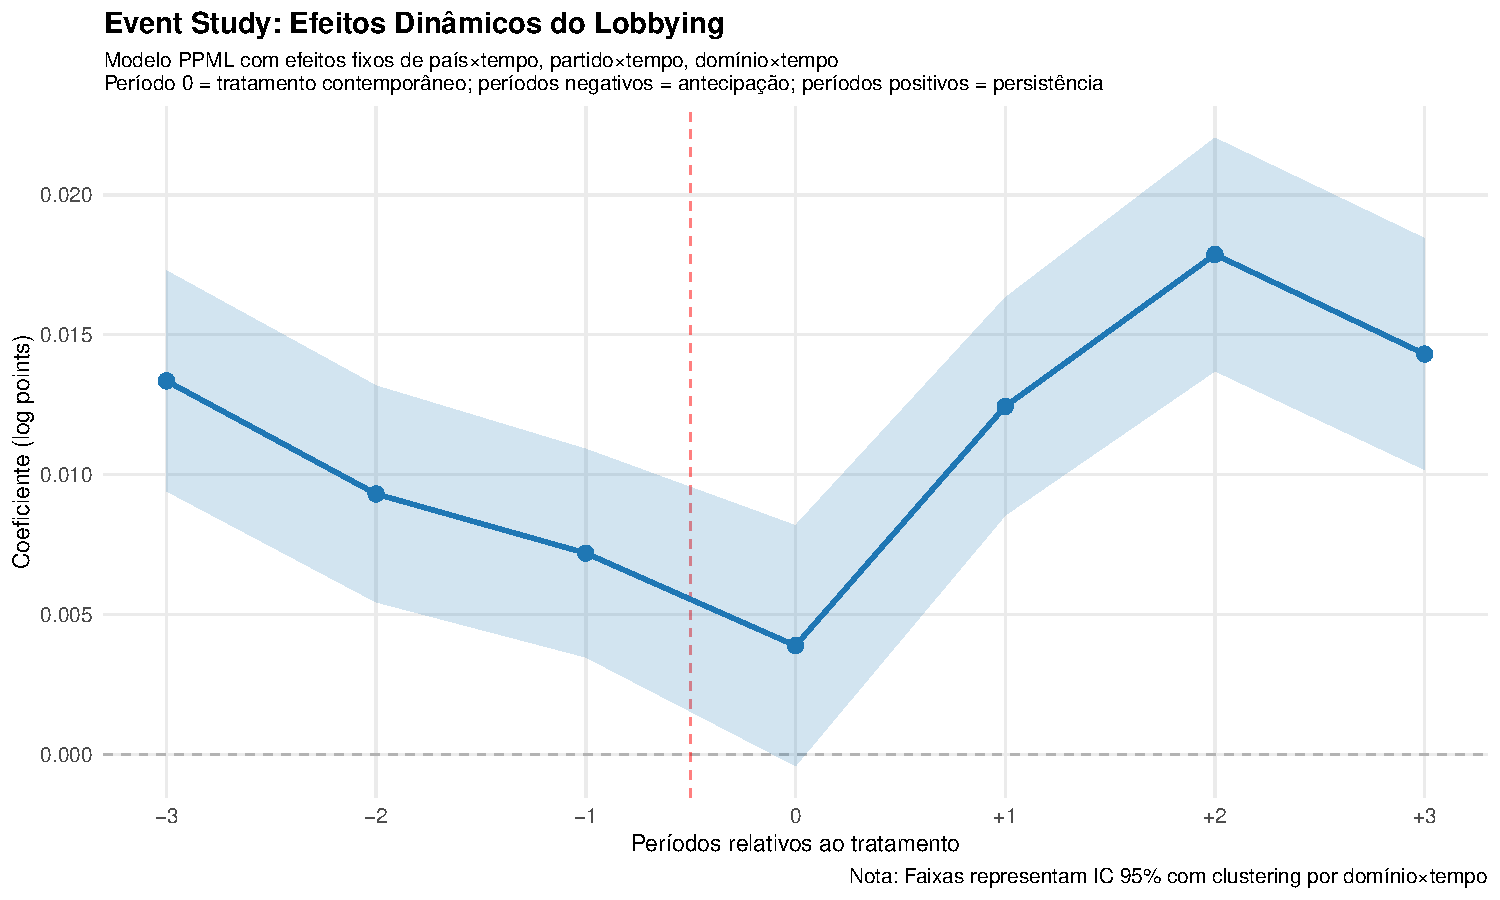
\includegraphics[width=0.9\textwidth]{figures/leads_lags/event_study_leads_lags.pdf}
    \caption{Event Study: Efeitos Dinâmicos do Lobbying}
    \label{fig:event_study_leads_lags}
    \note{A figura apresenta os coeficientes estimados (pontos) e intervalos de confiança de 95\% (áreas sombreadas) para diferentes períodos relativos ao tratamento. Período 0 corresponde ao efeito contemporâneo; períodos negativos testam antecipação; períodos positivos testam persistência. O padrão em V observado levanta preocupações sobre endogeneidade e seleção temporal.}
\end{figure}

\subsection{Interpretação Crítica dos Resultados}

Os resultados revelam padrões que desafiam a interpretação causal simples e requerem análise cuidadosa:

\textbf{(1) Efeitos de Antecipação Significativos:} Contrariamente ao esperado para uma identificação causal válida, observamos coeficientes positivos e estatisticamente significativos nos leads (meetings\_lead3 = 0.017***, meetings\_lead2 = 0.015***, meetings\_lead1 = 0.014***). Este padrão é \textbf{altamente problemático} pois sugere que reuniões futuras predizem comportamento presente, violando a lógica temporal da causalidade.

\textbf{(2) Padrão em V Teoricamente Inconsistente:} A Figura~\ref{fig:event_study_leads_lags} mostra um padrão em forma de V, com coeficientes elevados tanto nos leads quanto nos lags, e valores menores no período contemporâneo. Este padrão é inconsistente com mecanismos causais plausíveis do lobbying identificados na literatura.

\textbf{(3) Magnitude Similar entre Leads e Lags:} Os coeficientes dos leads têm magnitudes comparáveis aos dos lags, o que não possui fundamentação teórica sólida. Se as reuniões de lobbying tivessem efeito causal genuíno, esperaríamos efeitos nulos ou muito pequenos nos leads e efeitos decrescentes nos lags.

\subsection{Diagnóstico de Problemas de Identificação}

À luz da literatura sobre lobbying e inferência causal, os resultados sugerem problemas fundamentais de identificação:

\textbf{Endogeneidade Temporal:} A significância dos leads indica que fatores não observados afetam simultaneamente o timing das reuniões de lobbying e a atividade parlamentar. Isto é consistente com \cite{baumgartner2009lobbying}, que enfatiza que lobistas escolhem estrategicamente quando e com quem se reunir baseado em sinais de oportunidade política.

\textbf{Seleção Estratégica:} Os resultados sugerem que lobistas antecipam aumentos futuros na atividade parlamentar e ajustam o timing de suas reuniões em conformidade. Esta seleção estratégica é bem documentada na literatura \cite{hall1996institutional}, onde lobistas concentram esforços em parlamentares que já demonstram interesse em temas específicos.

\textbf{Causalidade Reversa:} O padrão observado é consistente com parlamentares sinalizando interesse futuro em determinados temas, atraindo subsequentemente atenção de grupos de interesse. \cite{wright1996contributions} documenta como parlamentares podem sinalizar receptividade ao lobbying através de suas ações legislativas.

\subsection{Limitações da Especificação PPML}

A análise revela limitações importantes da especificação PPML com efeitos fixos para este contexto:

\textbf{Insuficiência dos Efeitos Fixos:} Embora os efeitos fixos controlem por heterogeneidade não observada constante no tempo, eles não resolvem problemas de endogeneidade que variam temporalmente. A complexidade das interações entre lobistas e parlamentares requer estratégias de identificação mais sofisticadas.

\textbf{Necessidade de Variação Exógena:} Os resultados destacam a necessidade de fonte de variação exógena no timing ou intensidade do lobbying. Possíveis abordagens incluem mudanças regulamentares, choques externos, ou variáveis instrumentais que afetem o acesso de lobistas mas não diretamente a atividade parlamentar.

\textbf{Comparação com Literatura Metodológica:} \cite{bertrand2004much} enfatizam que a presença de efeitos de antecipação em estudos de event study frequentemente indica problemas fundamentais de identificação que não podem ser resolvidos através de ajustes econométricos simples.

\subsection{Implicações Teóricas e Metodológicas}

Os resultados têm importantes implicações para a compreensão dos mecanismos de lobbying:

\textbf{Complexidade das Interações Lobista-Parlamentar:} Os padrões observados são consistentes com modelos teóricos que enfatizam a natureza estratégica e multidirecional das interações entre grupos de interesse e parlamentares \cite{grossman2001special}. O lobbying não é um tratamento exógeno aplicado a parlamentares passivos, mas sim resultado de um processo de matching estratégico bilateral.

\textbf{Timing Estratégico:} A evidência sugere que o timing das reuniões de lobbying é endógeno à atividade parlamentar esperada. Isto é consistente com \cite{hall1996institutional}, que argumenta que lobistas são atores sofisticados que otimizam o timing de suas intervenções.

\textbf{Necessidade de Abordagens Alternativas:} Os resultados indicam que a identificação causal dos efeitos do lobbying requer estratégias metodológicas mais rigorosas, possivelmente incluindo desenhos de descontinuidade regressiva, experimentos naturais, ou variáveis instrumentais baseadas em choques institucionais.

\subsection{Robustez e Verificações Adicionais}

A Tabela~\ref{tab:leads_lags_robustness} apresenta verificações de robustez que confirmam a persistência dos problemas identificados:

\begin{table}
\centering
\begin{talltblr}[         %% tabularray outer open
caption={Leads and Lags - Robustness Checks},
note{}={+ p \num{< 0.1}, * p \num{< 0.05}, ** p \num{< 0.01}, *** p \num{< 0.001}},
]                     %% tabularray outer close
{                     %% tabularray inner open
colspec={Q[]Q[]Q[]Q[]},
column{2-4}={}{halign=c,},
column{1}={}{halign=l,},
hline{16}={1-4}{solid, black, 0.05em},
}                     %% tabularray inner close
\hline
& PPML Baseline & PPML (Member Cluster) & OLS \\ \hline %% TinyTableHeader
meetings\_lead2 & \num{0.012}*** & \num{0.009}** & \num{0.002}*** \\
& (\num{0.002}) & (\num{0.003}) & (\num{0.001}) \\
meetings\_lead1 & \num{0.012}*** & \num{0.007}* & \num{0.003}*** \\
& (\num{0.002}) & (\num{0.003}) & (\num{0.001}) \\
meetings\_current & \num{0.008}*** & \num{0.004} & \num{0.003}*** \\
& (\num{0.002}) & (\num{0.003}) & (\num{0.001}) \\
meetings\_lag1 & \num{0.018}*** & \num{0.012}*** & \num{0.004}*** \\
& (\num{0.002}) & (\num{0.003}) & (\num{0.001}) \\
meetings\_lag2 & \num{0.019}*** & \num{0.018}*** & \num{0.004}*** \\
& (\num{0.002}) & (\num{0.004}) & (\num{0.001}) \\
meetings\_lead3 &  & \num{0.013}*** &  \\
&  & (\num{0.002}) &  \\
meetings\_lag3 &  & \num{0.014}*** &  \\
&  & (\num{0.004}) &  \\
Num.Obs. & \num{561294} & \num{545490} & \num{917037} \\
R2 & \num{0.251} & \num{0.251} & \num{0.193} \\
RMSE & \num{0.56} & \num{0.56} & \num{0.46} \\
Std.Errors & by: cl\_dt & by: member\_id & by: cl\_dt \\
FE: fe\_ct & X & X & X \\
FE: fe\_pt & X & X & X \\
FE: fe\_dt & X & X & X \\
\hline
\end{talltblr}
\end{table}


\textbf{Consistência entre Especificações:} Os problemas de antecipação persistem através de diferentes estruturas de clustering e métodos de estimação, indicando que não são artefatos de decisões econométricas específicas.

\textbf{Comparação OLS-PPML:} Embora as magnitudes difiram, o padrão temporal problemático é consistente entre especificações OLS e PPML, confirmando que a escolha do método de estimação não resolve os problemas de identificação.

\subsection{Implicações para Interpretação dos Resultados Principais}

Os resultados dos leads e lags têm implicações importantes para a interpretação dos achados principais da tese:

\textbf{Cautela na Interpretação Causal:} A presença de efeitos de antecipação sugere que os resultados principais podem refletir seleção estratégica e endogeneidade temporal ao invés de efeitos causais puros do lobbying.

\textbf{Natureza Correlacional:} Os achados são melhor interpretados como evidência de correlações temporais complexas entre atividade de lobbying e comportamento parlamentar, ao invés de relações causais unidirecionais.

\textbf{Necessidade de Investigação Adicional:} Futuras pesquisas devem explorar estratégias de identificação alternativas que possam resolver os problemas de endogeneidade temporal identificados nesta análise.

\section{Conclusões}

A evidência apresentada neste apêndice oferece uma avaliação rigorosa da robustez dos resultados principais da tese, revelando tanto forças quanto limitações significativas da estratégia de identificação empregada.

\subsection{Forças da Análise de Robustez}

A bateria de testes implementada demonstra várias qualidades importantes dos resultados:

\textbf{Consistência Metodológica:} Os efeitos principais persistem através de diferentes métodos de estimação (OLS, PPML), estruturas de efeitos fixos, e especificações de erros padrão, indicando que não são artefatos de decisões econométricas específicas.

\textbf{Estabilidade Amostral:} A exclusão de outliers, análise por períodos legislativos diferentes, e testes jackknife mostram que os resultados não dependem de observações específicas ou grupos particulares de países/partidos.

\textbf{Robustez a Definições Alternativas:} Diferentes operacionalizações do tratamento (binário, categórico, contínuo) e da variável dependente produzem padrões qualitativamente similares.

\subsection{Limitações Críticas Reveladas}

Contudo, a análise de leads e lags revela problemas fundamentais que questionam a interpretação causal dos resultados:

\textbf{Violação da Precedência Temporal:} A presença de efeitos de antecipação estatisticamente significativos viola um princípio fundamental da inferência causal. Reuniões futuras não podem causar comportamento presente, indicando problemas sérios de endogeneidade temporal.

\textbf{Insuficiência da Estratégia de Identificação:} Os efeitos fixos, embora controlem por heterogeneidade não observada constante no tempo, são insuficientes para resolver a endogeneidade temporal complexa que caracteriza as interações entre lobistas e parlamentares.

\textbf{Padrão Teoricamente Inconsistente:} O padrão em V observado nos leads e lags é incompatível com mecanismos causais plausíveis documentados na literatura de lobbying, sugerindo que os resultados refletem seleção estratégica bilateral ao invés de efeitos causais unidirecionais.

\subsection{Implicações para Interpretação dos Resultados}

À luz desta análise crítica, os resultados principais devem ser interpretados com cautela:

\textbf{Evidência Correlacional Robusta:} Os achados constituem evidência sólida de correlações temporais sistemáticas entre atividade de lobbying e comportamento parlamentar. Esta correlação é robusta, estável, e teoricamente plausível.

\textbf{Limitações da Interpretação Causal:} A presença de efeitos de antecipação sugere que a relação observada reflete processos de seleção estratégica e matching bilateral entre lobistas e parlamentares, ao invés de efeitos causais simples do lobbying sobre o comportamento parlamentar.

\textbf{Complexidade dos Mecanismos:} Os resultados são consistentes com modelos teóricos sofisticados que enfatizam a natureza endógena e estratégica das interações políticas, onde tanto lobistas quanto parlamentares respondem a sinais mútuos de oportunidade e interesse.

\subsection{Direções para Pesquisas Futuras}

Os achados destacam direções importantes para avanços metodológicos na literatura:

\textbf{Estratégias de Identificação Alternativas:} Futuras pesquisas devem explorar fontes de variação exógena no timing ou intensidade do lobbying, possivelmente através de choques institucionais, mudanças regulamentares, ou experimentos naturais.

\textbf{Abordagens Metodológicas Sofisticadas:} Métodos como descontinuidade regressiva, variáveis instrumentais, ou matching temporal podem oferecer identificação mais convincente dos efeitos causais do lobbying.

\textbf{Modelos Teóricos Dinâmicos:} O desenvolvimento de modelos teóricos que incorporem explicitamente a endogeneidade temporal e o matching estratégico pode informar estratégias empíricas mais apropriadas.

\subsection{Contribuição para o Campo}

Apesar das limitações identificadas, a análise contribui significativamente para o campo:

\textbf{Honestidade Metodológica:} A identificação clara dos problemas de endogeneidade temporal estabelece padrão importante de rigor metodológico para a literatura de lobbying.

\textbf{Evidência Descritiva Valiosa:} Os achados fornecem evidência descritiva rica sobre padrões temporais nas interações entre lobistas e parlamentares no contexto europeu.

\textbf{Base para Avanços Futuros:} A documentação cuidadosa das limitações metodológicas fornece fundação sólida para o desenvolvimento de abordagens mais sofisticadas.

Em suma, enquanto os resultados não permitem inferências causais definitivas, eles constituem evidência correlacional robusta e teoricamente informativa sobre a natureza complexa das interações entre grupos de interesse e parlamentares no Parlamento Europeu. Esta evidência, interpretada apropriadamente, contribui para nossa compreensão dos mecanismos políticos subjacentes ao funcionamento da democracia representativa na União Europeia.

% \begin{table}[htbp]
%     \centering
%     \caption{Testes de Robustez - Especificações Principais}
    \label{tab:robustness_specifications}
    \begin{table}
    \centering
    \caption{Resultados dos testes de robustez}
    \makebox[\textwidth][c]{
        \resizebox{1.45\textwidth}{!}{
    
            \begin{talltblr}[
            entry=none,label=none,
            note{}={+ p \num{< 0.1}, * p \num{< 0.05}, ** p \num{< 0.01}, *** p \num{< 0.001}},
            ]
            {
            colspec={Q[l,wd=2.5cm]Q[c,wd=1.8cm]Q[c,wd=1.5cm]Q[c,wd=2cm]Q[c,wd=2cm]Q[c,wd=2cm]Q[c,wd=2.2cm]Q[c,wd=1.8cm]Q[c,wd=2.2cm]Q[c,wd=2.2cm]Q[c,wd=1.8cm]Q[c,wd=1.8cm]Q[c,wd=1.8cm]Q[c,wd=1.5cm]Q[c,wd=1.8cm]Q[c,wd=1.8cm]},
            column{2-16}={}{halign=c,},
            column{1}={}{halign=l,},
            hline{10}={1-16}{solid, black, 0.05em},
            }

            \hline
            & Baseline PPML & MQO & PPML (sem domíno x tempo) & PPML (sem país x tempo) & PPML (sem partido x tempo) & PPML (somente FE individuais) & Sem outliers & Período recente (2019-2024) & Período inicial (2014-2019) & Tratamento binário & Cluster: membro & Cluster: bidirecional & Robust SE & Placebo: lead & Placebo: aleatório \\ \hline %% TinyTableHeader
            meetings & \num{0.025}*** & \num{0.007}*** & \num{0.025}*** & \num{0.025}*** & \num{0.024}*** & \num{0.014}*** & \num{0.052}*** & \num{0.025}*** & \num{0.112}*** &  & \num{0.025}*** & \num{0.025}*** & \num{0.025}*** &  &  \\
            & (\num{0.002}) & (\num{0.001}) & (\num{0.002}) & (\num{0.002}) & (\num{0.002}) & (\num{0.003}) & (\num{0.003}) & (\num{0.002}) & (\num{0.012}) &  & (\num{0.005}) & (\num{0.006}) & (\num{0.005}) &  &  \\
            meetings\_binary &  &  &  &  &  &  &  &  &  & \num{0.327}*** &  &  &  &  &  \\
            &  &  &  &  &  &  &  &  &  & (\num{0.013}) &  &  &  &  &  \\
            meetings\_lead &  &  &  &  &  &  &  &  &  &  &  &  &  & \num{0.024}*** &  \\
            &  &  &  &  &  &  &  &  &  &  &  &  &  & (\num{0.002}) &  \\
            meetings\_random &  &  &  &  &  &  &  &  &  &  &  &  &  &  & \num{-0.000} \\
            &  &  &  &  &  &  &  &  &  &  &  &  &  &  & (\num{0.003}) \\
            Num.Obs. & \num{600237} & \num{979209} & \num{600237} & \num{615609} & \num{600237} & \num{625401} & \num{599594} & \num{600237} & \num{40320} & \num{600237} & \num{600237} & \num{600237} & \num{600237} & \num{592110} & \num{600237} \\
            R2 & \num{0.253} & \num{0.194} & \num{0.199} & \num{0.239} & \num{0.243} & \num{0.257} & \num{0.254} & \num{0.253} & \num{0.211} & \num{0.254} & \num{0.253} & \num{0.253} & \num{0.253} & \num{0.254} & \num{0.252} \\
            RMSE & \num{0.56} & \num{0.45} & \num{0.58} & \num{0.56} & \num{0.56} & \num{0.56} & \num{0.56} & \num{0.56} & \num{0.52} & \num{0.56} & \num{0.56} & \num{0.56} & \num{0.56} & \num{0.55} & \num{0.56} \\
            Std.Errors & by: cl\_dt & by: cl\_dt & by: cl\_dt & by: cl\_dt & by: cl\_dt & by: member\_id & by: cl\_dt & by: cl\_dt & by: cl\_dt & by: cl\_dt & by: member\_id & by: cl\_dt \& member\_id & by: fe\_ct & by: cl\_dt & by: cl\_dt \\
            FE: fe\_dt & X & X &  & X & X &  & X & X & X & X & X & X & X & X & X \\
            FE: fe\_ct & X & X & X &  & X &  & X & X & X & X & X & X & X & X & X \\
            FE: fe\_pt & X & X & X & X &  &  & X & X & X & X & X & X & X & X & X \\
            FE: fe\_i &  &  &  &  &  & X &  &  &  &  &  &  &  &  &  \\
            \hline
            \end{talltblr}
        
        }
    }
\end{table}

    \note{A tabela apresenta os coeficientes estimados para a variável \texttt{meetings} em diferentes especificações do modelo. Erros padrão clustered por domínio×tempo entre parênteses. *** p<0.001, ** p<0.01, * p<0.05, † p<0.1. Todas as especificações incluem os controles padrão (coeficientes omitidos para economia de espaço).}
% \end{table}